\def\thoigian{60}%--Thời gian
\de{ĐỀ THI GIỮA HỌC KỲ II NĂM HỌC 2023-2024}{THPT Vạn Hạnh - TPHCM}
%Câu 1...........................
\begin{bt}%[1D6H2-2]%[Dự án đề kiểm tra Toán 10 GHKI NH23-24- Hồ Văn Trung]%[THPT Vạn Hạnh]
	\begin{enumEX}{1}
		\item Rút gọn $\sqrt[5]{x \cdot \sqrt[4]{x^3 \cdot \sqrt[3]{x^2}}}$.
		\item Cho $\log_3a=2$, tính giá trị $P=\log_{27} \left( a^3 \cdot \sqrt[5]{a^2}\right)$.
		\item Cho các số thực dương $a$, $b$ thỏa mãn $4\log_2a+3\log_2b=2$. Tính $a^4b^3$.
	\end{enumEX}
	\loigiai{
		\begin{enumEX}{1}
			\item $\sqrt[5]{x \cdot \sqrt[4]{x^3 \cdot \sqrt[3]{x^2}}} = \sqrt[5]{x} \cdot \sqrt[5]{\sqrt[4]{x^3}} \cdot \sqrt[5]{\sqrt[4]{\sqrt[3]{x^2}}} = \sqrt[5]{x} \cdot \sqrt[20]{x^3} \cdot \sqrt[60]{x^2}= x^{\frac{1}{5}} \cdot x^{\frac{3}{20}} \cdot x^{\frac{1}{30}} = x^{\frac{23}{60}}$.
			\item $P=\log_{3^3}\left( a^3 \cdot a^{\frac{2}{5}} \right) = \log_{3^3}a^{\frac{17}{5}} = \dfrac{17}{15} \log_3a = \dfrac{17}{15} \cdot 2 = \dfrac{34}{15}$.
			\item Ta có 
				\begin{eqnarray*}
					& &4\log_2a+3\log_2b=2\\
					&\Leftrightarrow&\log_2a^4+\log_2b^3=2\\
					&\Leftrightarrow&\log_2a^4b^3=2\\
					&\Leftrightarrow&a^4b^3=2^2=4.
				\end{eqnarray*}
	\end{enumEX}}
\end{bt}
%câu 2.......................
\begin{bt}%[1D6H3-2]%[Dự án đề kiểm tra Toán 10 GHKI NH23-24- Hồ Văn Trung]%[THPT Vạn Hạnh]
	Tìm tập xác định của hàm số $y=\log(3x^2-x-2)$.
	\loigiai{Điều kiện xác định $3x^2-x-2>0 \Leftrightarrow \hoac{&x<\dfrac{-2}{3}\\&x>1.}$\\
	Vậy tập xác định hàm số đã cho là $\mathscr{D}=(-\infty;\dfrac{-2}{3}) \cup (1;+\infty)$.}
\end{bt}
%câu 3.......................
\begin{bt}%[1D6H4-2]%[Dự án đề kiểm tra Toán 10 GHKI NH23-24- Hồ Văn Trung]%[THPT Vạn Hạnh]
	Giải các phương trình sau
	\begin{enumerate}
		\item $\log_4(-2x^2+x+16)=\log_4(x^2+x+4)$.
		\item $\log_3(x+8)=3$.
	\end{enumerate}
	\loigiai{
\begin{enumEX}{1}
	\item 
	Điều kiện xác định: $\heva{&-2x^2+x+16>0\\&x^2+x+4>0.}$
	\begin{eqnarray*}
	& &\log_4(-2x^2+x+16)=\log_4(x^2+x+4)\\
	&\Leftrightarrow &-2x^2+x+16=x^2+x+4\\ 
	&\Leftrightarrow &-3x^2+12=0\\ 
	&\Leftrightarrow &\hoac{&x=-2\\&x=2.}
	\end{eqnarray*}
	So với điều kiện xác định ta thấy $x=-2$ và $x=2$ thỏa mãn.\\
	Vậy $S=\{-2;2\}$.
	\item 
	Điều kiện xác định: $x+8>0 \Leftrightarrow x>-8$.\\
	$\log_3(x+8)=3 \Leftrightarrow x+8=27 \Leftrightarrow x=19$.\\
	So với điều kiện xác định ta thấy $x=19$ thỏa mãn.\\
	Vậy $S=\{19\}$.
\end{enumEX}}
\end{bt}
%Câu 4.............................
\begin{bt}%[1D6V2-2]%[Dự án đề kiểm tra Toán 10 GHKI NH23-24- Hồ Văn Trung]%[THPT Vạn Hạnh]
	Cho $a=\log_{25}3; \; b=\log_25$. Tính $\log_5 \dfrac{81}{16}$ theo $a$ và $b$.
	\loigiai{Ta có $a=\log_{25}3 \Leftrightarrow a=\dfrac{1}{2}\log_53 \Leftrightarrow 2a=\log_53$.\\
	Ta có $\log_5 \dfrac{81}{16}=\log_581-\log_516=4\log_53-4\log_52=4\log_53-\dfrac{4}{\log_25}=8a-\dfrac{4}{b}.$
	}
\end{bt}
%Câu 5...............................
\begin{bt}%[1D6H3-3]%[Dự án đề kiểm tra Toán 10 GHKI NH23-24- Hồ Văn Trung]%[THPT Vạn Hạnh]
	Vẽ đồ thị hàm số mũ $y=2^x$.
	\loigiai{
	Bảng giá trị
	\begin{center}
		\begin{tabular}{c|c|c|c|c|c}
			$x$ & $-2$ & $-1$ & $0$ & $1$ & $2$\\ \hline
			$y$ & $\dfrac{1}{4}$ & $\dfrac{1}{2}$ & $1$ & $2$ & $4$ 
		\end{tabular}
	\end{center}
	\begin{center}
		\begin{tikzpicture}[smooth,samples=300,>=stealth]
			\draw[->] (-2.5,0)--(2.5,0) node[below]{$x$};
			\draw[->] (0,-0.5)--(0,5.35) node[right]{$y$};
			\draw (0,0) node[below left]{$O$};
			\draw[domain=-2.45:2.4] plot(\x,{2^(\x)}) node[right]{$y=2^x$};
			\draw[dashed] (1,0)node[below]{\small$1$}--(1,2)--(0,2)node[left]{\small$2$}
			(2,0)node[below]{\small$2$}--(2,4)--(0,4)node[left]{\small$4$}
			(-1,0)node[below]{\small$-1$}--(-1,0.5)--(0,0.5)node[right =-4pt]{$\tfrac{1}{2}$}
			(-2,0)node[below]{$-2$}--(-2,0.25)--(0,0.25)
			;
			\node[left] at (0,1.15) {\small $1$};
			\fill (0,1) circle(1.5pt) (1,2) circle(1.5pt) (-2,0.25) circle (1.5pt) (-1,0.5) circle (1.5pt) (2,4) circle (1.5pt)
			;
		\end{tikzpicture}
	\end{center}
	}
\end{bt}
%Câu 6..............................
\begin{bt}%[1D6V4-6]%[Dự án đề kiểm tra Toán 10 GHKI NH23-24- Hồ Văn Trung]%[THPT Vạn Hạnh]
	Trong năm 2019, diện tích đất trồng rừng mới của tỉnh A là $1000$ ha. Giả sử diện tích rừng trồng mới của tỉnh A mỗi năm tiếp theo đều tăng $6\%$ so với diện tích rừng trồng mới của năm liền trước. Kể từ sau năm 2019, năm nào là năm đầu tiên của tỉnh A có diện tích rừng trồng mới trong năm đó đạt trên $1400$ ha?
	\loigiai{Gọi $A_n$ là diện tích đất trồng rừng mới của tỉnh A sau n năm kể từ năm 2019.\\
	Ta có $A_n=1000 \cdot \left( 1+6\%\right)^n$.\\
	Để diện tích đất trồng rừng mới của tỉnh A đạt trên $1400$ ha suy ra 
	\begin{eqnarray*}
		& &A_n>1400\\
		& \Leftrightarrow &1000 \cdot \left( 1+6\%\right)^n > 1400\\
		& \Leftrightarrow &\left( 1{,}06\right) ^n>1{,}4\\
		& \Leftrightarrow &n> \log_{1{,}06}1{,}4 \approx 5{,}77.
		\end{eqnarray*} 
	Vậy năm đầu tiên có diện tích đất trồng rừng mới đạt trên $1400$ ha là sau $6$ năm. Tức là vào năm $2025$.
	}
\end{bt}
%Câu 7.............................
\begin{bt}%[1H8H2-2]%[Dự án đề kiểm tra Toán 10 GHKI NH23-24- Hồ Văn Trung]%[THPT Vạn Hạnh]
	Cho hình chóp $S.ABCD$ đáy $ABCD$ là hình vuông, $SA \bot (ABCD)$.
	\begin{enumEX}{1}
		\item Chứng minh rằng $\triangle SBC$ vuông.
		\item Trong $\triangle SAB$ kẻ đường cao $AH$, trong $\triangle SAC$ kẻ đường cao $AK$, chứng minh rằng $SC \perp (AHK)$.
	\end{enumEX}
	\loigiai{\begin{center}
			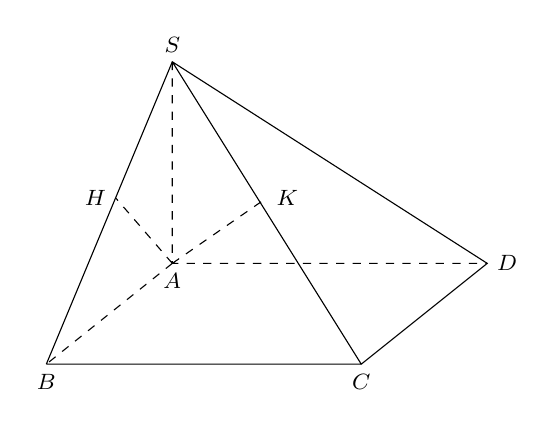
\begin{tikzpicture}[smooth,samples=300,scale=0.8,y=0.8cm,>=stealth,font=\footnotesize]
				\draw[dashed] (0,4)--(0,0)--(5,0) (0,0)--(-2,-2) (0,0)--(-0.9,1.3) (0,0)--(1.5,1.3);
				\draw (-2,-2)--(0,4)--(5,0)--(3,-2)--(0,4) (-2,-2)--(3,-2);
				\draw (0,0)node[below]{$A$} (0,4)node[above]{$S$} (-0.9,1.3)node[left]{$H$} (1.5,1.3) node[right]{$K$} (-2,-2)node[below]{$B$} (3,-2)node[below]{$C$} (5,0)node[right]{$D$};
			\end{tikzpicture}
	\end{center}
	\begin{enumEX}{1}
		\item Ta có $\heva{&BC \perp AB \;(ABCD \text{ là hình vuông})\\&BC \perp SA \;(SA \perp (ABCD))} \Rightarrow BC \perp (SAB) \Rightarrow BC \perp SB$.\\
		Do đó $\triangle SBC$ vuông tại B.
		\item Ta có $\heva{&AH \perp SB\; (AH \text{ là đường cao của tam giác }SAB )\\&AH \perp BC \;(BC \perp (SAB)).}\\ 
		\Rightarrow AH \perp (SBC) \Rightarrow AH \perp SC$.\\
		Mặt khác $AK \perp SC$ nên ta được $SC \perp (AHK)$.
\end{enumEX}	}
\end{bt}
%Câu 8................................
\begin{bt}%[1H8V2-3]%[Dự án đề kiểm tra Toán 10 GHKI NH23-24- Hồ Văn Trung]%[THPT Vạn Hạnh]
	Cho hình chóp $S.ABCD$ đáy $ABCD$ là hình vuông, $H$ là trung điểm $AB$, $SH \perp (ABCD)$, gọi $G$ là trực tâm của $\triangle SAB$. Chứng minh rằng $BG \perp SD$.
	\loigiai{\begin{center}
			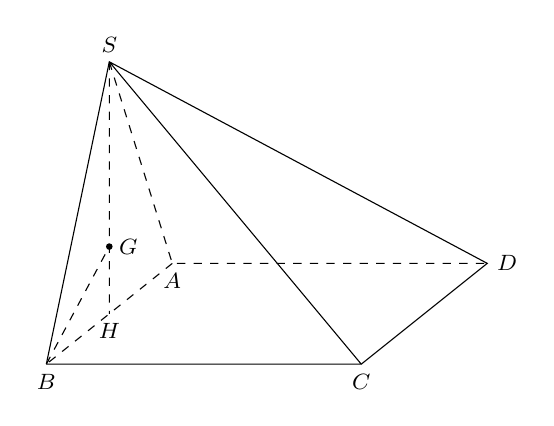
\begin{tikzpicture}[smooth,samples=300,scale=0.8,y=0.8cm,>=stealth,font=\footnotesize]
				\draw[dashed] (-1,4)--(0,0)--(5,0) (0,0)--(-2,-2) (-1,4)--(-1,-1) (-2,-2)--(-1,1/3);
				\draw (-2,-2)--(-1,4)--(5,0)--(3,-2)--(-1,4) (-2,-2)--(3,-2);
				\draw (0,0)node[below]{$A$} (-1,-1)node[below]{$H$} (-1,1/3)node[right]{$G$}
				(-1,4)node[above]{$S$} (-2,-2)node[below]{$B$} (3,-2)node[below]{$C$} (5,0)node[right]{$D$};
				\fill (-1,1/3) circle(1.5pt);
			\end{tikzpicture}
	\end{center}
	Tam giác $SAB$ có $G$ là trực tâm, suy ra $BG \perp SA$. (1)\\
	Ta có $\heva{&AD \perp AB\; (ABCD \text{ là hình vuông})\\&AD \perp SH\;(SH \perp (ABCD))} \Rightarrow AD \perp (SAB) \Rightarrow AD \perp BG$. (2)\\
	Từ (1) và (2) ta được $BG \perp (SAD) \Rightarrow BG \perp SD$. }
\end{bt}